\chapter{Lập trình là gì?}

\section{Các vấn đề lập trình}

Các vấn đề lập trình với từng ngôn ngữ

\subsection{Nhập môn}

\begin{lstlisting}
code/
├── 1. introduction
├── 2. syntax
├── 3. data structure
├── 4. oop
├── 5. networking
├── 6. os
├── 7. parallel
├── 8. event based
├── 9. error handling
├── 10. logging
├── 11. configuration
├── 12. documentation
├── 13. test
├── 14. ui
├── 15. web
├── 16. database
├── 17. ide
├── 18. package manager
├── 19. build tool
├── 20. make module
└── 21. production (docker)
\end{lstlisting}

\section{Introduction}

Installation (environment, IDE)

Hello world

Courses

Resources


\section{Syntax}

variables and expressions

conditional

loops and Iteration

functions

define, use

parameters

scope of variables

anonymous functions

callbacks

self-invoking functions, inner functions

functions that return functions, functions that redefined themselves

closures

naming convention

comment convention

\section{Cấu trúc dữ liệu}

Number

String

Collection

DateTime

Boolean

Object

\section{Lập trình hướng đối tượng}

Classes & Objects

Inheritance

Encapsulation

Abstraction

Polymorphism

For OOP Example: see Python: OOP

\subsection{Bài tập}

\textbf{Quản lý tài khoản ngân hàng}

\section{Networking}

REST (example with chat app sender, receiver, message)

\subsection{Bài tập}

Guess My Number Game

\section{GUI - Giao diện}

Quản lý hot girl

Quản lý truyện tranh

Create Analog Clock

Chương trình lịch âm dương

Chương trình học từ tiếng Anh

\section{Game}

\begin{itemize}
  \item Create Pong Game
  \item Create flappy bird
  \item Create Bouncing Game
\end{itemize}


\section{Cơ sở dữ liệu}

\subsection{Thử thách}


\section{How to ask a question}

Focus on questions about an actual problem you have faced. Include details about what you have tried and exactly what you are trying to do.

Ask about...

✔ Specific programming problems

✔ Software algorithms

✔ Coding techniques

✔ Software development tools

Not all questions work well in our format. Avoid questions that are primarily opinion-based, or that are likely to generate discussion rather than answers.

Don't ask about...

✖ Questions you haven't tried to find an answer for (show your work!)

✖ Product or service recommendations or comparisons

✖ Requests for lists of things, polls, opinions, discussions, etc.

✖ Anything not directly related to writing computer programs

\section{Các nguyên tắc lập trình}

Generic

KISS (Keep It Simple Stupid)

YAGNI

Do The Simplest Thing That Could Possibly Work

Keep Things DRY

Code For The Maintainer

Avoid Premature Optimization

Inter-Module/Class

Minimise Coupling

Law of Demeter

Composition Over Inheritance

Orthogonality

Module/Class

Maximise Cohesion

Liskov Substitution Principle

Open/Closed Principle

Single Responsibility Principle

Hide Implementation Details

Curly's Law

Software Quality Laws

First Law of Software Quality


\section{Các mô hình lập trình}

Main paradigm approaches 1

1. Imperative


Description:

Computation as statements that directly change a program state (datafields)

Main Characteristics:

Direct assignments, common data structures, global variables

Critics: Edsger W. Dijkstra, Michael A. Jackson

Examples: Assembly, C, C++, Java, PHP, Python

2. Structured

Description:

A style of imperative programming with more logical program structure

Main Characteristics:

Structograms, indentation, either no, or limited use of, goto statements

Examples: C, C++, Java, Python

3. Procedural

Description:

Derived from structured programming, based on the concept of modular programming or the procedure call

Main Characteristics:

Local variables, sequence, selection, iteration, and modularization

Examples: C, C++, Lisp, PHP, Python

4. Functional


Description:

Treats computation as the evaluation of mathematical functions avoiding state and mutable data

Main Characteristics:

Lambda calculus, compositionality, formula, recursion, referential transparency, no side effects

Examples: Clojure, Coffeescript, Elixir, Erlang, F#, Haskell, Lisp, Python, Scala, SequenceL, SML

5. Event-driven including time driven

Description:

Program flow is determined mainly by events, such as mouse clicks or interrupts including timer

Main Characteristics:

Main loop, event handlers, asynchronous processes

Examples: Javascript, ActionScript, Visual Basic

6. Object-oriented

Description:

Treats datafields as objects manipulated through pre-defined methods only

Main Characteristics:

Objects, methods, message passing, information hiding, data abstraction, encapsulation, polymorphism, inheritance, serialization-marshalling

Examples: Common Lisp, C++, C#, Eiffel, Java, PHP, Python, Ruby, Scala

7. Declarative

Description:

Defines computation logic without defining its detailed control flow

Main Characteristics:

4GLs, spreadsheets, report program generators

Examples: SQL, regular expressions, CSS, Prolog

8. Automata-based programming

Description:

Treats programs as a model of a finite state machine or any other formal automata

Main Characteristics:

State enumeration, control variable, state changes, isomorphism, state transition table

Examples: AsmL

\section{Testing}

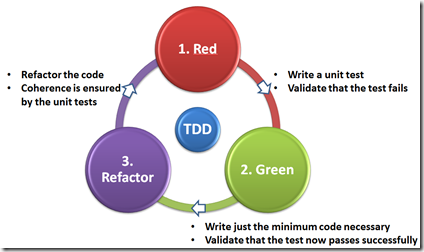
\includegraphics{programming/introduction/unit_test_tdd}

1. Definition 1 2

Test-driven development (TDD) is a software development process that relies on the repetition of a very short development cycle:

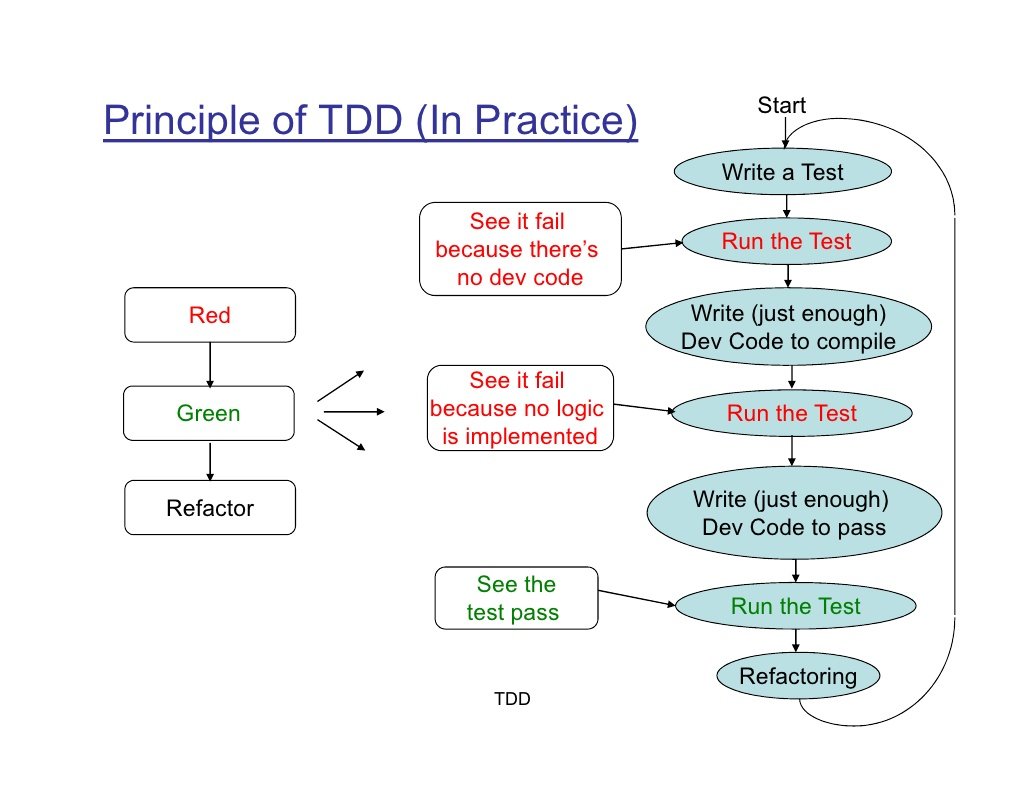
\includegraphics[width=\linewidth]{programming/introduction/tdd.jpg}

Step 1: First the developer writes an (initially failing) automated test case that defines a desired improvement or new function,

Step 2: Then produces the minimum amount of code to pass that test,

Step 3: Finally refactors the new code to acceptable standards.

Kent Beck, who is credited with having developed or 'rediscovered' the technique, stated in 2003 that TDD encourages simple designs and inspires confidence.

2. Principles 2

Kent Beck defines

Never with a single line of code unless you have a failing automated test.
Eliminate duplication
Red: (Automated test fail) Green (Automated test pass because dev code has been written) Refactor (Eliminate duplication, Clean the code)

3. Assertions & Assert Framework

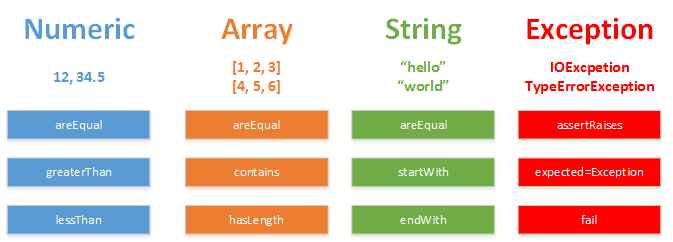
\includegraphics[width=\linewidth]{programming/introduction/tdd_assertion.png}

Assert that the expected results have occurred.
[code lang="java"] @Test public void test() { assertEquals(2, 1 + 1); } [/code]


4. Test Runners 3

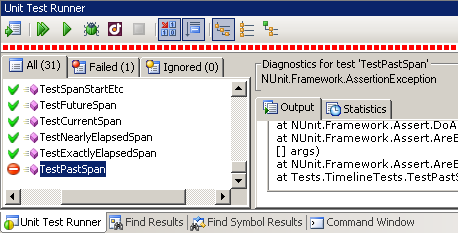
\includegraphics[width=\linewidth]{programming/introduction/tdd_test_runner.png}

When testing a large real-world web app there may be tens or hundreds of test cases, and we certainly don't want to run each one manually. In such as scenario we need to use a test runner to find and execute the tests for us, and in this article we'll explore just that.

A test runner provides the a good basis for a real testing framework. A test runner is designed to run tests, tag tests with attributes (annotations), and provide reporting and other features.

In general you break your tests up into 3 standard sections; setUp(), tests, and tearDown(), typical for a test runner setup.

The setUp() and tearDown() methods are run automatically for every test, and contain respectively:

The setup steps you need to take before running the test, such as unlocking the screen and killing open apps.
The cooldown steps you need to run after the test, such as closing the Marionette session.

5. Test Frameworks

Language	Test Frameworks
C++/VisualStudio	C++: Test
Web Service	rest-assured
Web UI	SeleniumHQ

\section{Logging}

Logging is the process of recording application actions and state to a secondary interface.


\includegraphics[width=\linewidth]{programming/introduction/logging}

Logging System

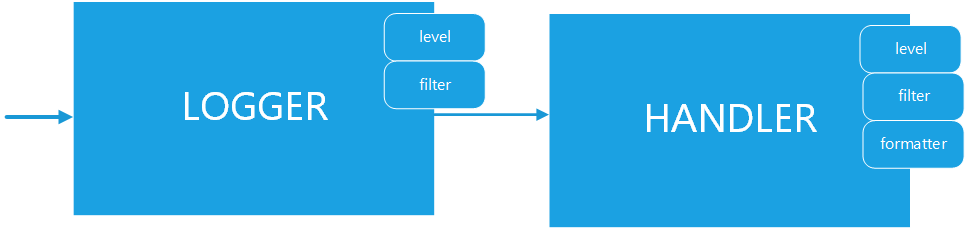
\includegraphics[width=\linewidth]{programming/introduction/logging_system}

Levels

Level	When it’s used
DEBUG	Detailed information, typically of interest only when diagnosing problems.
INFO	Confirmation that things are working as expected.
WARNING	An indication that something unexpected happened, or indicative of some problem in the near future (e.g. ‘disk space low’). The software is still working as expected.

ERROR

Due to a more serious problem, the software has not been able to perform some function.
CRITICAL	A serious error, indicating that the program itself may be unable to continue running.
Best Practices 2 4 5
Logging should always be considered when handling an exception but should never take the place of a real handler.
Keep all logging code in your production code. Have an ability to enable more/less detailed logging in production, preferably per subsystem and without restarting your program.
Make logs easy to parse by grep and by eye. Stick to several common fields at the beginning of each line. Identify time, severity, and subsystem in every line. Clearly formulate the message. Make every log message easy to map to its source code line.
If an error happens, try to collect and log as much information as possible. It may take long but it's OK because normal processing has failed anyway. Not having to wait when the same condition happens in production with a debugger attached is priceless.

\section{Lập trình hàm}

Functional
Without mutable variables, assignment, conditional

Advantages 1
Most functional languages provide a nice, protected environment, somewhat like JavaLanguage. It's good to be able to catch exceptions instead of having CoreDumps in stability-critical applications.
FP encourages safe ways of programming. I've never seen an OffByOne mistake in a functional program, for example... I've seen one. Adding two lengths to get an index but one of them was zero-indexed. Easy to discover though. -- AnonymousDonor
Functional programs tend to be much more terse than their ImperativeLanguage counterparts. Often this leads to enhanced programmer productivity.
FP encourages quick prototyping. As such, I think it is the best software design paradigm for ExtremeProgrammers... but what do I know.
FP is modular in the dimension of functionality, where ObjectOrientedProgramming is modular in the dimension of different components.
Generic routines (also provided by CeePlusPlus) with easy syntax. ParametricPolymorphism
The ability to have your cake and eat it. Imagine you have a complex OO system processing messages - every component might make state changes depending on the message and then forward the message to some objects it has links to. Wouldn't it be just too cool to be able to easily roll back every change if some object deep in the call hierarchy decided the message is flawed? How about having a history of different states?
Many housekeeping tasks made for you: deconstructing data structures (PatternMatching), storing variable bindings (LexicalScope with closures), strong typing (TypeInference), * GarbageCollection, storage allocation, whether to use boxed (pointer-to-value) or unboxed (value directly) representation...
Safe multithreading! Immutable data structures are not subject to data race conditions, and consequently don't have to be protected by locks. If you are always allocating new objects, rather than destructively manipulating existing ones, the locking can be hidden in the allocation and GarbageCollection system.

\section{Lập trình song song}

Paralell/Concurrency Programming
1. Callback Pattern 2
Callback functions are derived from a programming paradigm known as functional programming. At a fundamental level, functional programming specifies the use of functions as arguments. Functional programming was—and still is, though to a much lesser extent today—seen as an esoteric technique of specially trained, master programmers.

Fortunately, the techniques of functional programming have been elucidated so that mere mortals like you and me can understand and use them with ease. One of the chief techniques in functional programming happens to be callback functions. As you will read shortly, implementing callback functions is as easy as passing regular variables as arguments. This technique is so simple that I wonder why it is mostly covered in advanced JavaScript topics.

[code lang="javascript"] function getN(){ return 10; }

var n = getN();

function getAsyncN(callback){ setTimeout(function(){ callback(10); }, 1000); }

function afterGetAsyncN(result){ var n = 10; console.log(n); }

getAsyncN(afterGetAsyncN); [/code]

2. Promise Pattern 1 3
What is a promise?
The core idea behind promises is that a promise represents the result of an asynchronous operation.

A promise is in one of three different states:

pending - The initial state of a promise.
fulfilled - The state of a promise representing a successful operation.
rejected - The state of a promise representing a failed operation.
Once a promise is fulfilled or rejected, it is immutable (i.e. it can never change again).


\begin{lstlisting}[language=Javscript]
function aPromise(message){
  return new Promise(function(fulfill, reject){
    if(message == "success"){
      fulfill("it is a success Promise");
    } if(message == "fail"){
      reject("it is a fail Promise");
    }
  });
}
\end{lstlisting}

Usage:

\begin{lstlisting}[language=Javascript]
aPromise("success").then(function(successMessage){
  console.log(successMessage) }, function(failMessage){
  // it is a success Promise
  console.log(failMessage)
})
\end{lstlisting}

\begin{lstlisting}[language=Javascript]
aPromise("fail").then(function(successMessage){
  console.log(successMessage) }, function(failMessage){
  console.log(failMessage)
}) // it is a fail Promise
\end{lstlisting}

\section{IDE - Môi trường phát triển tích hợp}

An integrated development environment (IDE) is a software application that provides comprehensive facilities to computer programmers for software development. An IDE normally consists of a source code editor, build automation tools and a debugger. Most modern IDEs have intelligent code completion.

1. Navigation

Word Navigation Line Navigation File Navigation

2. Editing

Auto Complete Code Complete Multicursor Template (Snippets)

3. Formatting

Debugging
Custom Rendering for Object